\documentclass[]{spie}  %>>> use for US letter paper
%%\documentclass[a4paper]{spie}  %>>> use this instead for A4 paper
%%\documentclass[nocompress]{spie}  %>>> to avoid compression of citations
%% \addtolength{\voffset}{9mm}   %>>> moves text field down
%% \renewcommand{\baselinestretch}{1.65}   %>>> 1.65 for double spacing, 1.25 for 1.5 spacing 
%  The following command loads a graphics package to include images 
%  in the document. It may be necessary to specify a DVI driver option,
%  e.g., [dvips], but that may be inappropriate for some LaTeX 
%  installations. 
\usepackage[]{graphicx}
% % % These packages MBM inserted
\usepackage{caption} %This and Subcaption should allow me to use subcaptions in figures
\usepackage{subcaption}

\usepackage{float} % Allows putting an [H] in \begin{figure} to specify the exact location of the figure
\usepackage{wrapfig} % Allows in-line images such as the example fish picture
\usepackage{pdflscape} %allows pages to be landscape

\usepackage{lipsum} % Used for inserting dummy 'Lorem ipsum' text into the template

\usepackage{changes} %Allows the marking of changes
\definechangesauthor[color=blue]{Mark}

\title{Transverse strain response of in-fibre Fabry Perot microcavities} 

%>>>> The author is responsible for formatting the 
%  author list and their institutions.  Use  \skiplinehalf 
%  to separate author list from addresses and between each address.
%  The correspondence between each author and his/her address
%  can be indicated with a superscript in italics, 
%  which is easily obtained with \supit{}.

\author{Mark Manders, Matthew Partridge, Ricardo Correia, Stephen W James\supit{*} and Ralph P Tatam
%\author{Mark Manders\supit{a}, Dr Stephen James\supit{b} and Prof Ralph Tatam\supit{c}
\skiplinehalf
Engineering Photonics, School of Engineering, Cranfield University, Cranfield, Bedfordshire, MK43 0AL, UK %\\
%\supit{b}Affiliation2, Address, City, Country; \\
%\supit{C}Affiliation2, Address, City, Country
}

%>>>> Further information about the authors, other than their 
%  institution and addresses, should be included as a footnote, 
%  which is facilitated by the \authorinfo{} command.
\authorinfo{\supit{*} Stephen W James: E-mail: sw.james@cranfield.ac.uk, Telephone: 441232754623}
%\authorinfo{Further author information: (Send correspondence to Stephen W James)\\Stephen W James: E-mail: sw.james@cranfield.ac.uk, Telephone: 441232754623} %\\  B.B.A.: E-mail: bba@cmp.com, Telephone: +33 (0)1 98 76 54 32}
%%>>>> when using amstex, you need to use @@ instead of @
 

%%%%%%%%%%%%%%%%%%%%%%%%%%%%%%%%%%%%%%%%%%%%%%%%%%%%%%%%%%%%% 
%>>>> uncomment following for page numbers
% \pagestyle{plain}    
%>>>> uncomment following to start page numbering at 301 
%\setcounter{page}{301} 
 
\begin{document} 
\maketitle 

%%%%%%%%%%%%%%%%%%%%%%%%%%%%%%%%%%%%%%%%%%%%%%%%%%%%%%%%%%%%% 
\section*{Abstract}
In-fibre microcavity Fabry-Perot interferometers were constructed by splicing single mode fibre to polarisation maintaining photonic crystal fibre (PCF), with the air in the PCF pressurised to $5\pm0.005$bar. The response to transverse load was characterised, along with the influence of rotational orientation and the repeatability of the fabricaton process. A comparison of the microcavity response when coated in a fibre resin cube to uncoated was made. \replaced[id=Mark]{It was found that the features of the channelled reflected spectrum exhibited a blue wavelength shift with increasing applied transverse load}.
%>>>> Include a list of keywords after the abstract 

\keywords{Microcavity intrinsic Fabry-Perot interferometer, Photonic Crystal Fibre, Transverse Strain Sensor}

\section{Introduction}
An intrinsic Fabry-Perot interferometer (IFPI) consists of two in-fibre partial reflectors, with the region of fibre between them acting as the sensor\cite{2006MicroFP}. Extrinsic Fabry-Perot interferometers (EFPI) have been used in a large range of sensor applications such as structural health monitoring of dams, bridges and airplanes \cite{2006ProgFPI}. IFPIs can be embedded more easily in composites or used in harsh environments\cite{2006MicroFP}. Here we explore the use of microcavity IFPIs constructed at the junction between spliced single mode fibre and photonic crystal fibre (PCF)\cite{FibreBubble2011}. The fabrication of the device requires modification to the settings employed to achieve low-loss splice between different fibre types \cite{LowLossPCFsplice2012}. During the splice construction, the collapse of the holes in the heated section of the PCF causes air to flow into the splice, forming the void\cite{FibreBubble2011}. The void acts like a Fabry-Perot cavity with a characteristic channelled spectrum. This type of microcavity IFPI has been used as an axial strain sensor with a linear response in the range $0 \mu \epsilon$ to $1000 \mu \epsilon$ \cite{SpheFibreBub2012}. These devices have low thermal sensitivity ($1pm/ ^{0}C$) allowing a transverse sensor mostly immune to temperature change\cite{SpheFibreBub2012}. A comparison was made of the micocavity IFPIs uncoated and coated in a resin to explore the change in their sensitivity to axial strain, transverse stress and temperature change. A number of microcavity IFPIs were constructed to assess the consistency of the fabrication process.

\section{Method}
The microcavity Fabry-Perots were fabricated using a Fujikura 100P fusion splicer. The SMF fibre used was Fibercore SM750 and the polarisation maintaining photonic crystal fibre was NKT Photonics PM1550. The PM1550 was internally pressurised to $5.00\pm0.005$ bar during microcavity construction by connecting a Druck digital pressure indicator (DPI 601(IS)) to the proximal end of the fibre. The channelled spectrum produced by the microcavities was interrogated in reflection using an \replaced[id=Mark]{Ocean Optics S2000 spectrometer}, coupling the output an Ocean Optics SL-1 light source and a 50/50 coupler at $780nm$. The spectrometer had a resolution of \replaced[id=Mark]{$0.3nm$}, the peak position was resolved to less than this limit using a Spectrum Interrogation routine (SIR) developed in house. SIR is a Labview based peak fitting algorithm. The channelled spectrum of the microcavity consisted of a sinusoidal intensity pattern with a fringe visibility of \replaced[id=Mark]{$1.96$}. The periodicity is inversely proportional to the length of the microcavity. Figure \ref{fig:TypSpec} shows a typical channelled spectrum. The mean fringe separation of the cavities constructed was \replaced[id=Mark]{$16.5nm$} with a standard deviation of \replaced[id=Mark]{$5.2nm$}. This free spectral range of such a cavity length is \replaced[id=Mark]{$17.6\mu m$}. The mean length of the cavities constructed was \replaced[id=Mark]{$17.1\mu m$} with a standard deviation of \replaced[id=Mark]{$3.7\mu m$}. The measured cavity length corresponds well to the channelled spectrum periodicity. Three microcavities were interrogated by monitoring the shift in the position of peak channelled spectrum at $750nm$ as strain was applied. The cavities were photographed using an Olympus BX51 microscope to measure their dimensions, as shown in Figure \ref{fig:BubImages}.

\begin{figure}
\centering
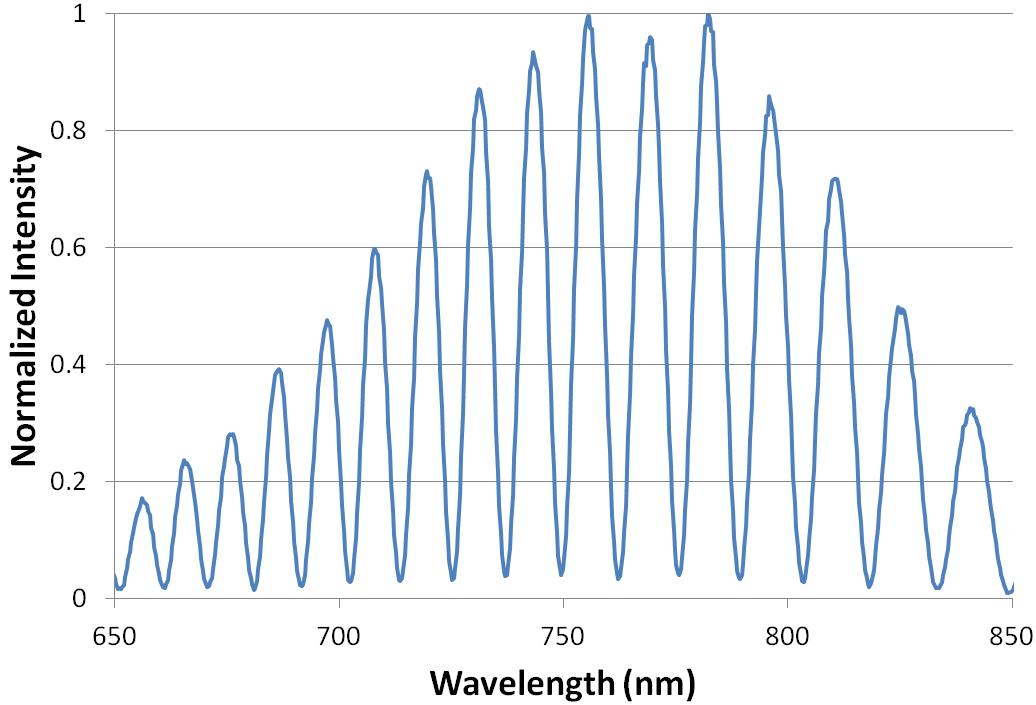
\includegraphics[width=0.51\linewidth]{./Pictures/TypSpec}
\caption{Typical channelled spectrum for an in-fibre microcavity Fabry Perot interferometer}
\label{fig:TypSpec}
\end{figure}

\begin{figure}[H]
\centering
	\begin{subfigure}{0.235\linewidth}
	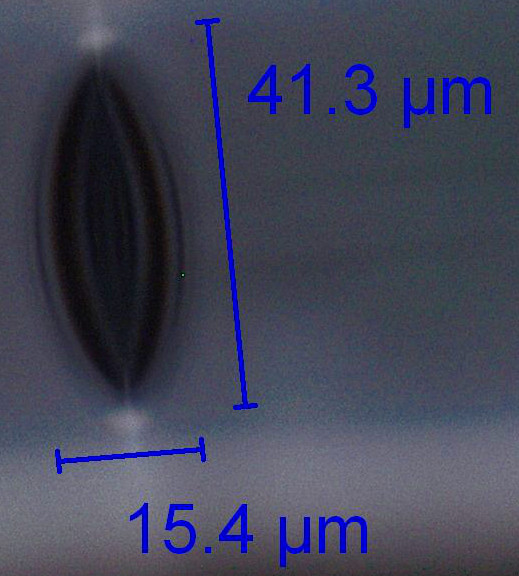
\includegraphics[width=0.6\linewidth]{./Pictures/Bub3}
	\caption{}
	\label{fig:Bub3Image}
	\end{subfigure}
	\begin{subfigure}{0.3\linewidth}
	\centering
	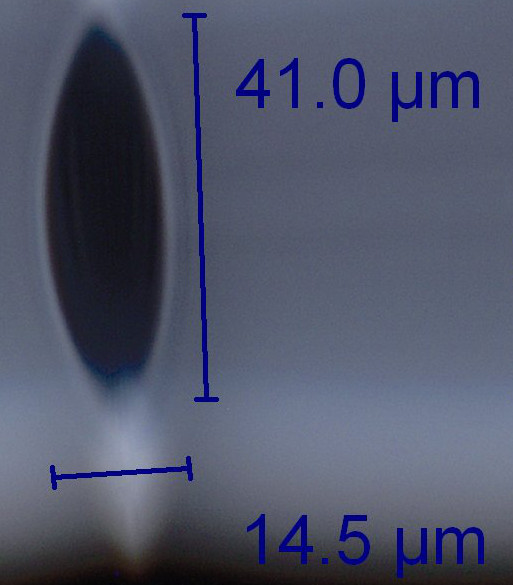
\includegraphics[width=0.6\linewidth]{./Pictures/Bub6}
	\caption{}
	\label{fig:Bub6Image}
	\end{subfigure}
	\begin{subfigure}{0.3\linewidth}
	\centering
	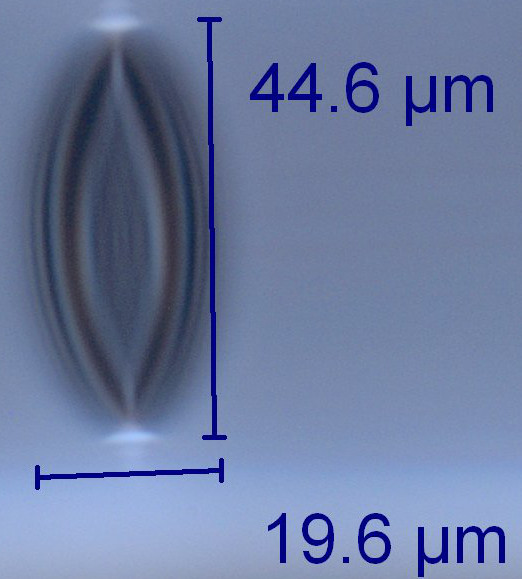
\includegraphics[width=0.6\linewidth]{./Pictures/Bub9}
	\caption{}
	\label{fig:Bub9Image}
	\end{subfigure}
\caption{Images of the microcavities taken with a Olympus BX51 microscope at 60x for microcavity 1 (a), microcavity 2 (b) and microcavity 3 (b)}
\label{fig:BubImages}	
\end{figure}
The uncoated microcavity IFPI was placed in a press when anisotropic stain was applied transverse to the axis of the fibre over a $2cm$ long region centred on the microcavity. The rotational dependence of the sensitivity to transverse loading was assessed by comparing the response with the fibre in two orthogonal orientations. The sensitivity of the micocavity to axial loading was also assessed by anchoring it to two optical mounts spaced by $151\pm 1mm$, with the distance between the anchoring points increased in increments of $20 \mu m$ from $0 \mu m$ to $200 \mu m$. The thermal response of the microcavity was assessed by heating with an electrical filament from $25^{0}C$ to $125^{0}C$. Once a microcavity's response to axial strain, transverse stress and temperature change was recorded it was coated in a resin cube $2mm$ by $2mm$ by $2mm$. The measurements were repeated. This was done for three microcavities.
\section{Results}

\section{Conclusion}

%%%%%%%%%%%%%%%%%%%%%%%%%%%%%%%%%%%%%%%%%%%%%%%%%%%%%%%%%%%%%

\section*{Acknowledgements}
M.M would like to acknowledge the support of an EPRSC DTA and the Authors would like to acknowledge support from EPSRC Platform grant EP/H02252x/1. 

%\cite{FibreBubble2011, SpheFibreBub2012, LowLossPCFsplice2012, 2006ProgFPI, 2006MicroFP, 2013EigenDecompFP}


\bibliographystyle{spiebib}   %>>>> makes bibtex use spiebib.bst
\bibliography{Literature140515}   %>>>> bibliography data in report.bib

\end{document}